\documentclass{article}
\usepackage[utf8]{inputenc}
\usepackage{hyperref}
\usepackage{graphicx}
\usepackage{fixltx2e}
\usepackage{bm}
\setlength{\parskip}{1em}
\usepackage[margin=1.0in]{geometry}
\usepackage{pgfplots}
\usepackage{subfig}
\usepackage{url}
\usepackage{amsmath}
\usepackage[
    backend=bibtex, 
    natbib=true,
    style=numeric,
    sorting=none
    ]{biblatex}
\addbibresource{ref.bib}
\setcounter{biburllcpenalty}{7000} % required to prevent long URLs from exceeding the page margin
\setcounter{biburlucpenalty}{8000}
\pgfplotsset{width=10cm,compat=1.9}
\usepgfplotslibrary{external}
\tikzexternalize

\title{Lab 4: Weight Training\\
  \large ECSE 421: Embedded Systems \\ Department of Electrical and Computer Engineering \\ McGill University \\ Version 1.1}
\author{Adam Cavatassi and Jeremy Cooperstock}
\date{Winter 2018}

\begin{document}

\maketitle

\section{Introduction}
You have previously been provided with the data set that was used to train Position-NET. In this lab, you will learn how to carry out such training of a simple, fully connected neural network, to reconstruct the inference engine from Lab 3. These instructions will guide you through the basics of neural network training, including the back propagation algorithm. All setup and lab instructions have been verified to work with LabVIEW 2016 on the PCs in Trottier Building Room 5090. 

\section{Neural network training}

Recall from Lab 3 that neural networks are trained to make predictions by being presented with examples from a labeled training set, consisting of a set of inputs, or features, and the corresponding output, over a number of iterations. Such an artificial neuron calculates the dot product of an input vector, $\mathbf{x}$ of dimension $N$, with a weight vector, $\mathbf{w}$ as

\begin{equation}
    net = \sum\limits_{i=0}^{N-1} w_i x_i + b
\end{equation}

where $b$ is an optional bias offset. 


In essence, Equation (1) determines on which side of a decision boundary, defined by the weights, the input vector lies.  Such a neuron can thus be used as a linear classifier. The calculated value, $net$ may then be passed through an activation function, $\Sigma$. For the original perceptron algorithm from 1957, this activation function is the simple step function. 
Other activation functions, such as the sigmoid, $\sigma(net)$ and hyperbolic tangent function, $\tanh(net)$, are often used, and for deep learning, a popular function is the \textbf{re}ctified \textbf{l}inear \textbf{u}nit, or \textit{reLU}, which calculates $\mathrm{reLU}(net) = max(0, net)$.


Most data sets are made up of a large number of data points, or training examples, consisting of an input vector and a target class. The training examples are fed through an untrained neural \mathbf{net}work that outputs values based on the input vector. The error between the expected output, or target, $\mathbf{t_n}$, and the computed output, or prediction, $\mathbf{y_n}$,
of the n\textsubscript{th} training example, can be measured using a differentiable cost function. A cost function used to measure error can be defined as a function of the \mathbf{net}work weights, $\mathbf{W}$. Two popular loss functions are the \textit{mean squared error} function:

\begin{equation}
\label{eq:mse}
    J_n(\mathbf{W}) = \frac{1}{2}(\mathbf{y_n} - \mathbf{t_n})^2
\end{equation}

and the \textit{cross-entropy error} function:

\begin{equation}
\label{eq:cee}
   J_n(\mathbf{W}) = -[\mathbf{y_n}\log{\mathbf{t_n}} + (1-\mathbf{y_n})\log{(1-\mathbf{t_n})}]
\end{equation}

The loss is an indicator of how well trained the \mathbf{net}work is. The goal from this point is to optimize the weights of the \mathbf{net}work in order to minimize the loss for all training examples.

The weights for a given \mathbf{net}work architecture are unknown at first. As such, it is sufficient for the weights to be initialized with a random number of uniform distribution such that $\mathbf{W} \in [-1,1]$. Once all weights in the \mathbf{net}work are randomly assigned, we can begin the training.

An intuitive approach to minimize the loss would be to take the derivative, or gradient, of the loss function with respect to the weights, equate the derivative to zero, and solve for the weights. This method is not feasible since the feed-forward \mathbf{net}work is too complex, and there is no closed-form solution. However, an optimization can be approximated using a process known as gradient descent, which updates the \mathbf{net}work weights iteratively by stepping along the error gradient towards a local minimum according to the equation:

\begin{equation}
\label{eq:gd}
   \mathbf{W}_{new} = \mathbf{W}_{old} - \alpha \nabla J(\mathbf{W})
\end{equation}

where $\nabla J(\mathbf{W})$ is the average error gradient with respect to the \mathbf{net}work weights over all training examples, and $\alpha$ is the learning rate. The learning rate is a hyper parameter that dictates the size of the steps in each iteration. Fig.~\ref{fig:gd} presents a simple visualization of the method in which, for purposes of illustration, the loss function relates to only a single weight.  After each iteration, the weights are modified to reduce the error.  As such, the gradient can have high dimensionality, and the local minimum found using gradient descent is usually not the global minimum. The starting point of the error is dependent on the initially chosen weight values, which can result in inconsistent optimization results. 

\begin{figure}[h]
\centering
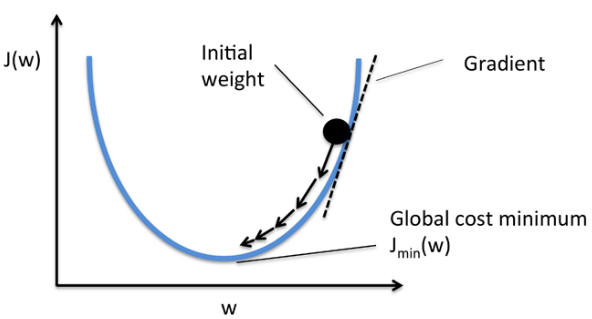
\includegraphics[scale=0.6]{figs/gd.png}
\caption{Visualization of gradient descent. \cite{gd}}
\label{fig:gd}
\end{figure}

Fig. \ref{fig:gd_3d} illustrates the same process dependent on multiple weights, in which two different initial values for the weights lead to very different local minima of the gradient, neither of which are necessarily the global minimum. 

\begin{figure}[h]
\centering
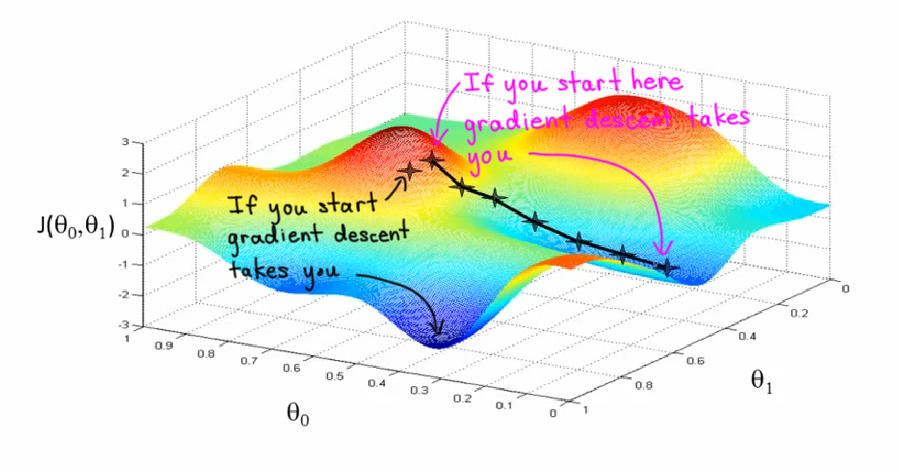
\includegraphics[scale=0.5]{figs/gd_3d.jpeg}
\caption{Multi-dimensional gradient descent, illustrating the consequences of random weight initialization. \cite{gd_3d}}
\label{fig:gd_3d}
\end{figure}


Since subsequent layers after the input layer produce activations, each of those layers will have an associated loss gradient. During neural \mathbf{net}work training, the weights between each pair of layers must be updated separately.  However, we cannot compute the loss at layer $k$ without first computing the loss at layer $k + 1$. For this reason, we must propagate the error from the output layer back to the hidden layers through the gradients. This process is known as a backwards pass, or back-propagation. To compute the gradient with respect to all weights between layer $k$ and layer $k + 1$, we must find the derivative of the loss function with respect to the \mathbf{net}work weights:

\begin{equation}
\label{eq:grad}
   \nabla J(\mathbf{W}) = \frac{\partial J(\mathbf{W})}{\partial \thinspace \mathbf{W}}
\end{equation}

This derivative can be expanded by the chain rule to define the gradient:

\begin{equation}
\label{eq:chain}
   \nabla J(\mathbf{W}) = \frac{\partial J(\mathbf{W})}{\partial \mathbf{W}} = \frac{\partial J(\mathbf{W})}{\partial \mathbf{y}} \frac{\partial \mathbf{y}}{\partial \mathbf{net}} \frac{\partial \mathbf{net}}{{\partial \mathbf{W}}}
\end{equation}

where $\mathbf{y}$ and $\mathbf{\mathbf{net}}$ are the activation and dot product, respectively, of each node in the corresponding layer. The weight vectors 
are then adjusted by subtracting the gradients, multiplied by the learning rate, as defined by Eq.~\ref{eq:gd}. A backwards pass consists of computing the gradient for each layer successively, starting with the output layer and working towards the input layer. The backwards pass is completed when all weights have been updated. A full training iteration consists of a forward pass, calculation of the error, followed by a backwards pass, over all training examples.

However, the backwards pass does not need to be applied over each of the training examples, individually. For efficiency, the gradient $\nabla J(\mathbf{W})$ can be computed using the average error from all training examples, or by selecting a subset of training examples at random and using those to calculate the average error instead. This modified approach is called stochastic gradient descent, and the selected subset of training samples is known as a batch. Training with this method can still be effective with a batch size as small as a single example. The benefit of using a smaller batch of examples is that gradient computation can be faster. However, this approach can result in noisier weight updates, and thus can require more training time to converge to a local minimum. 

Training time is also affected by the learning rate. The learning rate is always set to a value less than 1, typically $\ll 1$, e.g., 0.001. Determining an optimal learning rate for a given machine learning application requires some experimentation. A smaller learning rate leads to smaller steps along the gradient, which results in longer training time. A larger learning rate can result in big steps that may overshoot a local minimum, potentially leading to longer convergence times. This effect is visualized in Fig.~\ref{fig:lr}. The training process continues to iterate until a sufficiently low error has been reached. 

\begin{figure}[h!]
\centering
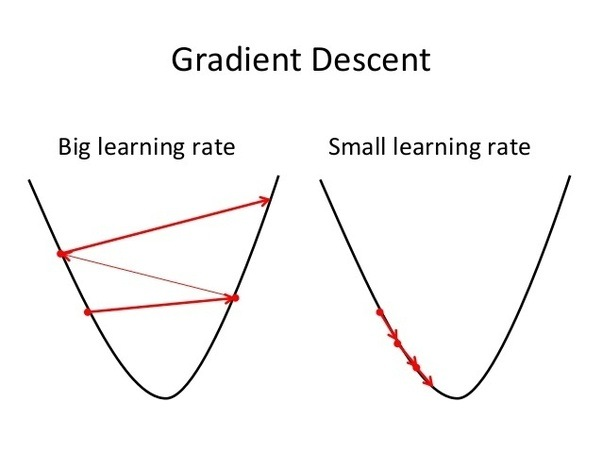
\includegraphics[scale=0.6]{figs/lr.jpeg}
\caption{A comparison of large and small learning rates. \cite{lr}}
\label{fig:lr}
\end{figure}

\begin{figure}[h!]
\centering
\hspace{3cm} 
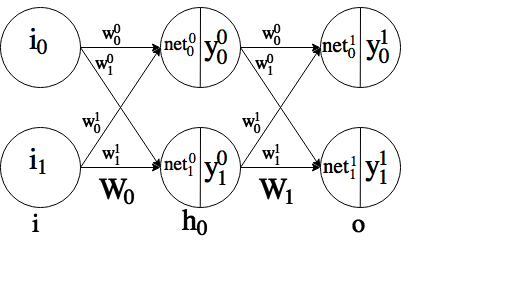
\includegraphics[scale=0.7]{figs/bp_ex.png}
\caption{Example neural network.}
\label{fig:bp_ex}
\end{figure}

\begin{figure}[h!]
\centering
\hspace{0.5cm} 
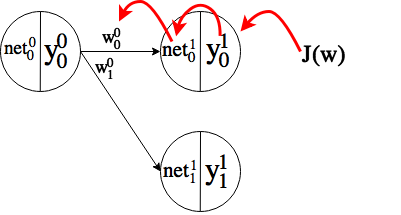
\includegraphics[scale=0.7]{figs/weight_update.png}
\caption{Gradient computation for the output layer using chain rule.}
\label{fig:wu}
\end{figure}


\subsection{Gradient computation example}

Let's look at an example of gradient descent computation. Consider the simple neural network in Fig. \ref{fig:bp_ex} with 2 inputs, 2 nodes in the hidden layer, and 2 nodes in the output layer. Both the hidden layer and output layer use the sigmoid activation function, and the mean squared error cost function to train the netwwork. The output from this netwwork is the vector $\mathbf{y^1}$, and the target values are the vector $\mathbf{t}$. To compute the gradient $\nabla J(\mathbf{W_1})$ for the output layer and update the weights in matrix $\mathbf{W_1}$, we can use the chain rule as outlined in Equation \ref{eq:chain}. Note that the subscripts for the weight matrices $\mathbf{W_k}$ refer to layer $k$. All superscripts for vectors $\mathbf{net^k}$ and $\mathbf{y^k}$ refer to layer $k$, and all subscripts for vector elements $net^k_j$ and $y^k_j$ refer to node $j$. For each weight matrix, the individual edge weights are represented in the format $w^i_j$, where $i$ is the source node and $j$ is the destination node.



The derivative of $\frac{\partial J(\mathbf{W_1})}{\partial \mathbf{y^1}}$ is of course:

\begin{equation}
\label{}
   \frac{\partial J(\mathbf{W_1})}{\partial \mathbf{y^1}} = \frac{\partial}{\partial \mathbf{y^1}}\bigg[\frac{1}{2}(\mathbf{y^1} - \mathbf{t})^2\bigg] = \mathbf{y^1} - \mathbf{t}
\end{equation}

Next, we need the derivative $\frac{\partial \mathbf{y^1}}{\partial \mathbf{\mathbf{net}}\mathbf{^1}}$:

\begin{equation}
\label{}
   \frac{\partial \mathbf{y^1}}{\partial \mathbf{net}\mathbf{^1}} = \frac{\partial}{\partial \mathbf{net}\mathbf{^1}}\bigg[\sigma(\mathbf{net}\mathbf{^1})\bigg] = \sigma(\mathbf{net}\mathbf{^1})(1 - \sigma(\mathbf{net}\mathbf{^1}))
\end{equation}

Lastly, the derivative $\frac{\partial \mathbf{net}\mathbf{^1}}{\partial \mathbf{W_1}}$:

\begin{equation}
\label{}
   \frac{\partial \mathbf{net}\mathbf{^1}}{\partial \mathbf{W_1}} = \frac{\partial}{\partial \mathbf{W_1}}\bigg[ 
   \begin{matrix} w_0^0y_0^0 + w_0^1y_1^0 \\ w_0^0y_0^0 + w_1^1y_1^0 \end{matrix} 
   \bigg] = \bigg[\begin{matrix} y_0^0 & y_1^0 \end{matrix}\bigg] = \mathbf{y^0} \thinspace ^\top
\end{equation}

Finally, the complete gradient can be written as:

\begin{equation}
\label{}
   \nabla J(\mathbf{W_1}) = \big[ (\mathbf{y^1} - \mathbf{t})\sigma(\mathbf{net}^1)(1 - \sigma(\mathbf{net}^1))\big] \times \mathbf{y^0} \thinspace ^\top = \mathbf{\boldsymbol{\delta}_{1}} \times \mathbf{y^0} \thinspace ^\top
\end{equation}

Note that the term $\mathbf{y^0} \thinspace ^\top$ is in transposed form. This equation should result in a gradient matrix in the same shape as the weight matrix that we intend to modify. This gradient can now be used to update weight matrix $\mathbf{W_1}$ using Equation~\ref{eq:gd}. Similarly, the gradient for the hidden layer can be computed by modifying the $\mathbf{\boldsymbol{\delta}_{k}}$ term:

\begin{equation}
\label{}
   \nabla J(\mathbf{W_0}) = \mathbf{\boldsymbol{\delta}_{0}} \times \mathbf{i} \thinspace ^\top
\end{equation}

where $\mathbf{i}$ is the input vector to the neural network, and $\mathbf{\boldsymbol{\delta}_0}$ is the delta loss vector for the hidden layer $\mathbf{h_0}$, which is dependent on the delta loss from the proceeding layer (ie. the layer closer to the output of the network). The delta loss for any layer $\mathbf{h_k}$ can be generalized as such:

\begin{equation}
\label{}
   \mathbf{\boldsymbol{\delta}_k} = \frac{\partial J(\mathbf{W_k})}{\partial \mathbf{y^k}} \frac{\partial \mathbf{y^{k}}}{\partial \mathbf{\boldsymbol{\alpha}^k}} = \begin{cases}
            (\mathbf{y^k} - \mathbf{t})\sigma(\mathbf{net}^k)(1 - \sigma(\mathbf{net}^k)) & \text{if output layer} \\
            (\mathbf{W_{k+1}} \times \mathbf{\boldsymbol{\delta}_{k+1}})\sigma(\mathbf{net}^k)(1 - \sigma(\mathbf{net}^k) & \text{if hidden layer}
        \end{cases}
\end{equation}

\section{Training Position-Net}

It is now up to you to train \textit{Position-Net} yourself using the given data set, consisting of 1500 training samples with 500 samples for each of the three classes. The input vectors from the training set should match yours, so that $\mathbf{i} = [a_x, a_y, a_z, \theta_{roll}, \theta_{pitch}]$. The output targets are not one-hot encoded. Recall that Position-Net consists of five input nodes, a single hidden layer with eight nodes, and an output layer of three nodes. 

Position-Net, shown in Fig.\ref{fig:position_net}, was originally trained using the sigmoid activation function and mean squared error cost function. Using the given data set, you need to acquire your own weights to recreate the inference engine you built in Lab 3. The network should be able to accurately guess at which of the three positions the myRIO board is in based on the data supplied to the input nodes. You need to build the back-propagation algorithm yourself. You are not allowed to re-use the weights from the previous lab, and your are not allowed to use any machine learning libraries from National Instruments or any other programming environment.  

\begin{figure}[h]
\centering
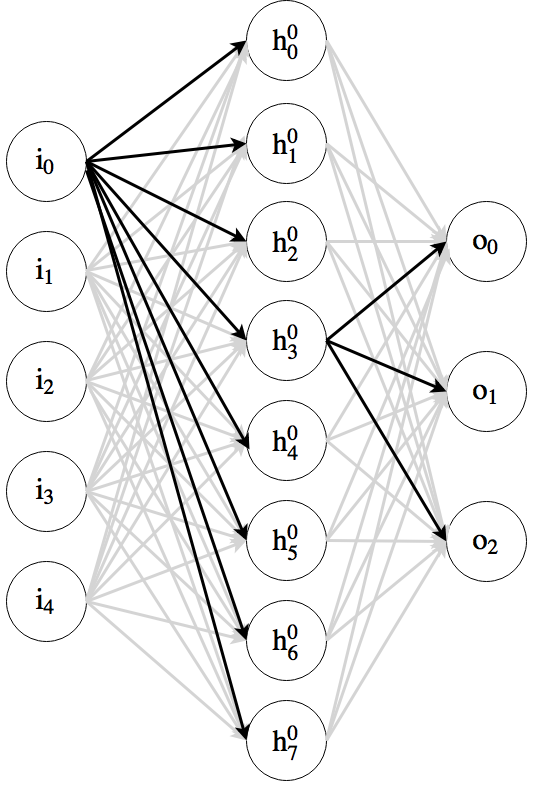
\includegraphics[scale=0.3]{figs/position_net.png}
\caption{Position-Net, consisting of 5 input nodes, 8 hidden nodes, and 3 output nodes.}
\label{fig:position_net}
\end{figure}

The data set is stored in two separate .csv files: one for the inputs, and one for the output targets. Use the provided VI to import the input data and targets into your project. Ensure that the data is properly loaded into the project and into the shared variables that your myRIO board can access. If you are unsure of how to do this, consult the importing instruction from Lab 3. Everything should work the same way for this lab. 

There are a few important points to keep in mind when training a neural network.  First, training tends to perform poorly when the back propagation algorithm iterates over the entire data set while it is sorted by target. The reason for this is the network will spend many iterations training its weights with respect to a single class. When the network moves on to the cluster of data which consists of only the second class, it will begin training for that class and "forget" the first class. There are two ways to combat this. The first is to shuffle the data set before beginning training. This way, each iteration has a high probability of seeing a different class, allowing the network to evenly train on all classes. The second method to perform more uniform training is to use stochastic gradient descent, as outlined above. Using one training example at random to update the weights can be surprisingly effective. 

Second, it is important to avoid over-training the network (otherwise known as "over-fitting"), since this results in reduced generalization ability, and thus, a poor classifier when exposed to previously unseen data.  The way to avoid such over-fitting is to set aside a portion of the collected data as a "validation set" that is not used for updating the weights of the network.  Instead, during training, performance of the network is evaluated regularly on the validation set, and training is stopped when error on  validation data begins to increase, as seen in Fig. \ref{fig:val}.  Both the training and validation sets should ideally be sampled randomly from the collected data.  

\begin{figure}[h]
\centering
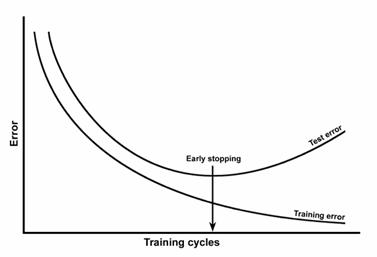
\includegraphics[scale=1]{figs/val.jpg}
\caption{An example of validation set error increasing when a neural network begins to overfit the training data.  Training should stop at the "early stopping point" to avoid overfitting. \cite{val}}
\label{fig:val}
\end{figure}

A typical validation split can be between 15\% and 25\% of the data set.  Since you will begin with randomly initialized weights, your resulting weight matrices will differ from the ones supplied to you for the previous lab. It is entirely possible that your inference engine will thus perform better or worse than the one provided to you previously.

Be sure to consider a highly modular and efficient implementation. It will make your final project much easier. Try to find as many ways to reduce training time as possible. This can be done any number of ways, including optimizing the learning rate, making use of stochastic gradient descent, utilizing as many LabVIEW components as possible. Implementing your own embedded C/MATLAB scripts can bypass many of the optimizations National Instruments has made for you. You may even consider using the on-board FPGA or fixed-point data representation to speed up computations. The sky is the limit! You may also want to create a VI on the PC target to save your weights to a .csv file if you find a good set of weights that you do not want to lose when you close LabVIEW.

\section{Submission requirements}

For this lab, you will be required to submit a .zip file containing your project file, all VI files that are part of your project, and screenshots of both the final block diagram and final front panel for all VIs. The front panel of your training VI should include a plot of training and validation set errors over time. Be sure that one of your screenshots includes this functionality in action. You will also be required to submit a URL to a private YouTube video with a maximum length of 180 seconds that demonstrates the full functionality of the network training (including an error plot), followed by the inference engine that you trained in real-time. If you saved a set of weights that perform well, you may use those to demonstrate the inference engine provided that you {\bf also} demonstrate that your system is able to learn the weights. This concession is being made because the random nature to the weight initialization means that you may not always obtain a good training result every time you run your code. You should demonstrate the best possible inference engine you are able to achieve, convincing the viewer that your your weights were synthesized from your code and not reused from the previous lab. Your network outputs are still LED0, LED1, and LED2 on the myRIO board. Show that each position is clearly recognized by the neural network after training, as indicated by the LEDs.


\printbibliography

\onecolumn

\end{document}
